\documentclass[12pt, leqno]{article} %% use to set typesize
\input{common}

\begin{document}
\hdr{2018-06-22}

\section{Collaborative filtering and other stories}

The usual story behind {\em collaborative filtering} is that each user
in a system rates some items (movies, books, etc), with different
items for each user.  We want to predict the missing ratings for a
user in order to recommend things she would like.  But there are many
other applications that fit the same pattern.  For example,
in modern genomics application, we may have incomplete (or corrupted)
information for the DNA sequences for many individuals, and want to
fill in the missing parts.  In image analysis, we may have many
pictures of the same background, but with different parts missing or
corrupted due to noise or occlusions.  And in many other settings,
we have data that can be expressed in matrix form, and we would like
to estimate the missing entries.  We refer to this general problem
as {\em matrix completion}, though in other settings it is sometimes
called {\em imputation}.

Before we dive into our main topic, let's consider a few toy models
that we could use for collaborative filtering (for example).
Throughout, we will let $A$ be the ``true'' data, of which
we observe a subset of entries with index pairs $\Omega$.
The projection $P_{\Omega}(A)$ is the matrix with
\[
  P_{\Omega}(A)_{ij} =
  \begin{cases}
    a_{ij}, & (i,j) \in \Omega \\
    0, & \mbox{otherwise}
  \end{cases}
\]
Our goal is to choose a model $M$ from some parametric family
in order to minimize some loss function.  Several loss functions are
plausible, but for today we will focus on the squared error loss
\[
  \phi(\mu)
  = \frac{1}{2} \|P_{\Omega}(M)\|_F^2
  = \frac{1}{2} \sum_{(i,j) \in \Omega} (a_{ij}-\mu)^2.
\]

Perhaps the simplest model is to assume that there is some
``baseline'' rating that all items get, and the excursions from that
baseline are just noise.  In matrix terms, we write this model as
$M = \mu ee^T$, where $\mu$ is the baseline rating and $e$
denotes a vector of all ones.  The minimum squared error loss occurs
at the sample mean $|\Omega|^{-1} \sum_{(i,j) \in \Omega} a_{ij}$.
While it is easy to fit, though, this model is nearly useless in its
simplicity; certainly it would not tell us how to recommend one unread
book over another!

Moving up one more level of complexity, consider a model of
the form
\[
  M = \mu ee^T + be^T + ec^T,
\]
where the vectors $b \in \bbR^m$ and $c \in \bbR^n$ represent
uniform adjustments for each user and item, respectively.
Minimizing the least squares loss for this model is still
a relatively simple linear least squares problem, but even
here we run into two issues:
\begin{itemize}
\item
  The problem does not have a unique solution!  In fact, the space of
  minimizers is at least two dimensional: if $\mu, b, c$ is one
  minimizer for the least squares loss, so is
  $\mu + \alpha, b + \beta e, c - (\alpha + \beta) e$ for
  any $\alpha, \beta$.
\item
  The least squares problem is large; if we lay it out in matrix form,
  the matrix will have size $|\Omega| \times (1+m+n)$ where $m$ and
  $n$ are the number of users and items, respectively.
\end{itemize}
The first issue is only a problem if we are unaware of it.  There are
many possible solutions, but all predict the same ratings.  We could
choose a unique solution by adding auxiliary conditions; for example,
we might insist that the entries of $b$ and $c$ both sum to zero.
Or we could regularize the problem, or we could choose a method that
finds {\em a} solution to the least squares problem and declare
victory.  The second issue is only an issue if we insist on using
factorization-based direct methods.  An alternative would be to use
an iterative method: an alternating least squares method of the type
we discussed last time will converge R-linearly, and LSQR will
converge even faster.

The second model we considered is still not useful for providing
user-specific recommendations; rather, it will predict the
same {\em relative} ranking of items for every user, even if the
numerical scores are biased in a user-specific way.  We can get
actual useful recommendations if we go one further step in model
complexity and choose a low-rank model
\[
  M = XY^T.
\]
This model is {\em nonlinear} in the parameters (the entries of $X$
and $Y$).  Like the previous model, it is over-parameterized ---
there are multiple choices of $X$ and $Y$ that will provide the
same solution.  And on top of this, it is nonconvex!  Nonetheless,
we have successfully dealt with these issues before, and we will
deal with them here as well.

\section{Alternating iteration}

There are many ways to factor a rank $k$ matrix in outer product
form, and so the model $A \approx M = XY^T$ is not unique.  In order
to avoid completely wild choices of $X$ and $Y$ with very large
or very small coefficients, we might decide to regularize the
fitting problem to penalize the case when $X$ or $Y$ have large
Frobenius norm.  That is, we seek to minimize
\[
  F(X,Y) =
    \frac{1}{2} \|P_{\Omega}(A)-P_{\Omega}(XY^T)\|_F^2 +
    \frac{\lambda}{2} \left( \|X\|_F^2 + \|Y\|_F^2 \right)
\]
for some regularization parameter $\lambda$.  Let
$R = P_{\Omega}(A-XY^T)$, and notice that
\begin{align*}
  \langle \delta R, R \rangle_F
  &= \langle P_{\Omega}(-(\delta X) Y^T - X(\delta Y)^T ) R, R \rangle_F \\
  &= -\langle (\delta X) Y^T, R \rangle_F -\langle X (\delta Y)^T, R \rangle_F \\
  &= -\tr(Y (\delta X)^T R)-\tr((\delta Y) X^T R) \\
  &= -\tr((\delta X)^T RY)-\tr((R^TX)^T \delta Y) \\
  &= -\langle \delta X, RY \rangle_F - \langle \delta Y, R^T X \rangle_F.
\end{align*}
Taking variations of $F$ therefore gives
\[
  \delta F =
    \langle \delta X, \lambda X - R   Y \rangle_F +
    \langle \delta Y, \lambda Y - R^T X \rangle_F.
\]
Thus, at a stationary point $\delta F = 0$,     
the matrices $X$ and $Y$ must span matching left and right
singular subspaces\footnote{%
  Just as an invariant subspace is spanned by (possibly generalized)
  eigenvectors, a singular subspace is spanned by singular vectors.
}
of $R$.

If we observe all the data (i.e. $R=A-XY^T$ with no projection),
then for $X$ and $Y$ to span singular subspaces of $R$, they must
span singular subspaces of $A$, and therefore can be written neatly
in terms of the SVD of $A$.  In this case, one global minimizer is
\[
  X = U_k \sqrt{s_{\lambda}(\Sigma_k)}, \quad Y = V_k \sqrt{s_{\lambda}(\Sigma_k)}
\]
where $U_k$, $V_k$, and $\Sigma_k$ are truncated SVD factors for
$A$ associated with the largest $k$ singular values,
and $s_{\lambda}(\sigma) = [\sigma-\lambda]_+$,
with $s_{\lambda}(\Sigma_k)$ denoting the function $s_{\lambda}$
applied to each singular value.  Note that when $\lambda = 0$,
we recover the SVD-based optimal rank $k$ approximation from
Eckart-Young!  Of course, the problem becomes
trickier when we have only partial data.

We can minimize $F$ through a wide variety of iterations.
For example, we might decide to tackle the problem with a method like
stochastic gradient descent, updating based on sampling a few ratings
at a time.  But, as with NMF, we can also approach the minimization
via alternating iteration:
\begin{align*}
  X^{k+1} &= \operatorname{argmin}_X F(X,Y^k) \\
  Y^{k+1} &= \operatorname{argmin}_Y F(X^{k+1},Y).
\end{align*}
Each of these minimization steps can be further decomposed
into a collection of small linear least squares problems.
For example, to compute a row $x_i^T$ of the updated $X$
factor in the first step, we would solve a regularized
least squares problem of the form
\[
  x_i = \operatorname{argmin}_x
  \frac{1}{2} \| Y_{\Omega_i} x - a_{\Omega_i} \|_2^2 +
  \frac{\lambda}{2} \|x\|^2,
\]
where $\Omega_i = \{ j : (i,j) \in \Omega \}$,
$Y_{\Omega_i}$ represents the corresponding rows of $Y$,
and $a_{\Omega_i}$ represents the vector of ratings for
item $i$ (i.e.~the numbers $a_{ij}$ for $j \in \Omega_i$).
We solve similar regularized least squares problems to update $Y$.

Assuming we solve each of these least squares problems anew by a
factorization method at each step, the overall cost per iteration is
$O(|\Omega| k^2)$ per step.  In principle we could reduce the cost to
$O(|\Omega| k)$ after an initial step where we pre-computed the
relevant factorizations, though with a cost of an extra $O(|\Omega|
k)$ in storage.

\section{The nuclear norm trick}

An alternative to optimizing factors is to optimize the matrix;
that is, we would like to directly minimize the error subject to
a rank constraint, or possibly a rank penalty.  Unfortunately,
the rank of a matrix is not even a continuous function of the
matrix entries, which makes it hard to optimize.  But we can get
something that is almost what we want and is nice to optimize\footnote{%
  ``Nice to optimize'' in this case should be read as ``yields a
  convex optimization problem, so there are no local minimizers and we
  can draw on a good toolkit of numerical methods.''  The problem is
  still large and non-smooth, so ``nice'' does not necessarily mean
  ``easy.''}
by instead penalizing the {\em nuclear norm} of the model matrix:
\[
\phi(M) =
  \frac{1}{2} \|P_{\Omega}(A) - P_{\Omega}(M)\|_F^2 +
  \lambda \|M\|_*, \quad
  \|M\|_* \equiv \sum_i \sigma_i(M).
\]

\begin{figure}
  \begin{center}
  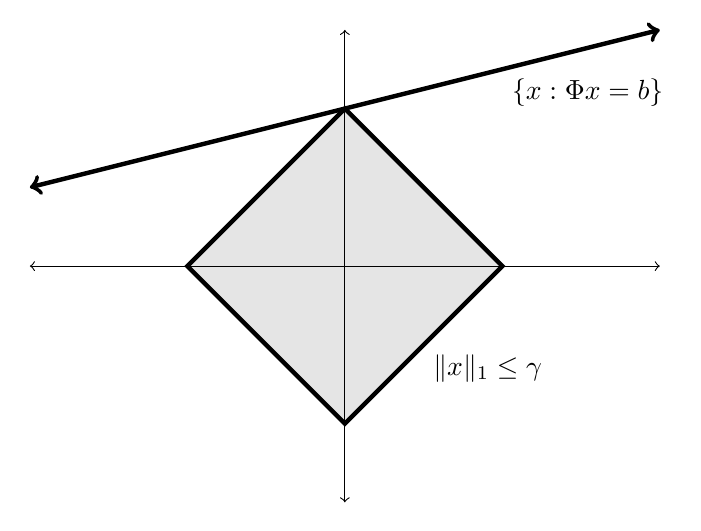
\begin{tikzpicture}
    \draw[<->,ultra thick] (-4,1) -- (4,3);
    \draw node at (2,2.5) [below right] {$\{x : \Phi x = b \}$};
    \draw[ultra thick, fill=black!10]
    (-2,0) -- (0,-2) -- (2,0) -- (0,2) -- cycle;
    \draw node at (1,-1) [below right] {$\|x\|_1 \leq \gamma$};
    \draw[<->] (-4,0) -- (4,0);
    \draw[<->] (0,-3) -- (0,3);
  \end{tikzpicture}
  \end{center}
  \caption{Intuition behind 1-norm minimization for compressive
    sensing.}
  \label{fig:cs}
\end{figure}

To understand why the nuclear norm trick works, it is helpful to first
look at the analogous trick in a simpler setting.  Suppose we want to
solve an underdetermined system of equations
\[
  \Phi x = b
\]
where $\Phi \in \bbR^{m \times n}$ with $m < n$.  This equation admits
a whole $(n-m)$-dimensional affine space of solutions, but suppose we
know that there is one solution hidden within the space that is
sparse, with only $k$ nonzero elements.  How might we find those $k$
elements?  The sparsity $\|x\|_0 = \#\mbox{nonzeros in $x$}$ is
obviously not a continuous function of $x$, and minimizing the
sparsity subject to constraints is not an easy problem.  What we can
do, though, is to minimize $\|x\|_1 = \sum_i |x_i|$ subject to the
constraints, and this works almost as well -- this is the idea behind
much of {\em compressed sensing}, as well as the lasso regularization
that we discussed two weeks ago.  In the affine space of solutions to
the linear equations $\Phi x = b$, a minimal 1-norm solution occurs at
the intersection of the space and the smallest possible 1-norm ball.
This intersection tends to occur at a corner of the ball,
corresponding to a sparse solution $x$ (see Figure~\ref{fig:cs}).
The nuclear norm is the Ky-Fan 1-norm, i.e.~a matrix norm
defined as the 1-norm of the vector of singular values; and just as
minimizing the 1-norm over an affine set of vectors tends to
find the sparsest element in the set, minimizing the nuclear norm
over an affine set of matrices tends to find the lowest rank matrix
in the set.

A useful building block for minimizing the nuclear-norm regularized
objective $\phi$ is the solution to the {\em proximal problem}:
\[
S_\lambda(A) =
  \operatorname{argmin}_M \frac{1}{2} \|A-M\|^2 + \lambda \|M\|_*.
\]
If $A = U \Sigma V^T$, the solution to this problem is
\[
  S_{\lambda}(A) = U s_{\lambda}(\Sigma) V^T,
\]
where $s_{\lambda}(\sigma) = [\sigma-\lambda]_+$ is exactly the same
``soft thresholding'' operator we saw at the start of the previous
section.  Hence, in the case that $A$ has at most $k$ singular values
larger than $\lambda$, the solution to the nuclear norm proximal
problem is equivalent to
\[
\mbox{minimize }
  \frac{1}{2} \|A-XY^T\|_F^2 + \frac{\lambda}{2} (\|X\|_F^2 + \|Y\|_F^2)
\]
where $M = XY^T$.  In fact, a similar result holds when we look at
only part of the data matrix: the nuclear norm regularized
optimization and the optimization of the factorized form with
Frobenius regularization on the factors yield {\em the same} model
predictions when the factor size $k$ in the latter problem is at least
as large as the rank observed in the nuclear norm problem.

The SVD formulation of the proximal problem suggests an
algorithm for solving the nuclear norm regularized optimization
known as SVD thresholding (SVDT):
at each iterate, use the current model to fill in the missing data
entries, then solve a proximal problem with the estimated full data.
In symbols, we have:
\[
  M^{j+1} = S_{\lambda}(M^{j} + P_{\Omega}(A-M^{j})).
\]
This may initially seem impractically expensive for large data
matrices, since we have to compute an SVD at each step.  However, we
only expect to have to compute a small number of singular values
greater than the threshold $\lambda$ at each step, which we can
compute using a Lanczos-type algorithm that relies only on
matrix-vector products with the matrix
$M^{j} + P_{\Omega}(A-M^{j})$.  We generally suppose $M^{j}$
will be low rank, and the matrix $P_{\Omega}(A-M^{j})$ is sparse;
consequently, the matrix-vector products required for the Lanczos
iteration can be performed very efficiently.

We like the nuclear norm optimization problem because it is convex,
and we need not worry about local minima.  We like the factorized
optimization problem because the iterates have fixed size, and we need
not worry about the possibility that a full rank (or high-rank) $M^{j}$
at some intermediate step will ruin the complexity of our solve.
The fact that these formulations are equivalent when the factors are
wide enough gives us some flexibility in going back and forth between
them, and hope for getting the best of both worlds.

\subsection{Robust PCA}

The nuclear norm trick is useful for more than just matrix completion.
Another problem amenable to the same trick is the {\em robust PCA}
problem of splitting a matrix into a sum of sparse and low rank parts:
\[
  A \approx M+E
\]
where $M$ is low rank and $E$ sparse.  Using the nuclear norm as a
proxy for low rank and the (vector) one-norm as a proxy for sparsity,
we have the formulation
\[
  \mbox{minimize } \|M\|_* + \mu \|E\|_1 \mbox{ s.t. } A = M+E.
\]
The ingredients for a common algorithm to solve this problem are
similar to the ingredients we have seen before: alternating iteration,
together with thresholding operations for solving proximal problems.
Of course, because this is a constrained problem, we also need some
Lagrange multipliers.  In order to deal with these efficiently, it
is helpful to use the trick of adding
a constraint violation penalty to the objective:
\[
  \mbox{minimize } \|M\|_* + \mu \|E\|_1 + \frac{1}{2\beta}
  \|A-(M+E)\|_F^2 \mbox{ s.t. } A = M+E
\]
for some $\beta$.  This does not change the solution to the
optimization problem at all, but compared to the Lagrangian for the
original problem, it is easier to find the critical points for
the resulting {\em augmented Lagrangian}
\[
  L(M,E,\Lambda) =
    \|W\|_* + \mu \|E\|_1 +
    \langle \Lambda, M+E-A \rangle_F +
    \frac{1}{2\beta} \|M+E-A\|_F^2.
\]
If we apply the alternating iteration solver idea, we can compute
\begin{align*}
  M^{j+1} &= S_{\beta}(A-E^j - \beta \Lambda^j) \\
  E^{j+1} &= s_{\beta \mu} (A-M^{j+1}-\beta \Lambda^j) \\
  \Lambda^{j+1} &= \Lambda^j - \frac{\delta_j}{\beta} (A-M^{j+1}-E^{j+1})
\end{align*}
where $\delta_k$ is a step size parameter.  Here $S_{\beta}$ refers to
the singular value shrinkage / thresholding operator that we have seen
previously, while $s_{\beta \mu}$ refers to an elementwise shrinkage
operator
\[
  s_{\lambda}(z) = \operatorname{sgn}(z) [|z|-\lambda]_+.
\]
This iterative thresholding algorithm is by no means the fastest
modern algorithm for robust PCA, but other more sophisticated
algorithms are built from similar basic operations.

\section{When should this work?}

In addition to work on developing algorithms, there has been an
enormous amount of theoretical work to determine when matrix
completion and robust PCA techniques based on nuclear norm and one
norm objectives will actually ``work'': that is, assuming there is an
underlying ``true'' low-rank factorization or low-rank-plus-sparse
decomposition, will that decomposition be recovered by these
optimization techniques?  The answer is yes, the true decomposition
will be recovered with high probability assuming that there are enough
measurements, well enough spread about, and that an ``incoherence''
condition is satisfied.  The incoherence condition rules out
pathological cases where, for example, we have a rank $k$ matrix with
only $k$ nonzeros (none of which are observed).  If the information in
the low-rank matrix is not ``spread out'' enough that we can see it
with the observations $\Omega$, there is little hope that we can
recover it!  However, the technical conditions under which we know how to
prove exact recovery still appear to be somewhat conservative, and
there are cases where these methods work better than we know how to
prove.

\end{document}
